%% The following is a directive for TeXShop to indicate the main file
%%!TEX root = diss.tex

%-------------------------------------------------------------------------
%-------------------------------------------------------------------------
%-------------------------------------------------------------------------

\chapter{Reflection and Conclusion}
\label{ch:conclusions}

%-------------------------------------------------------------------------
%-------------------------------------------------------------------------
%-------------------------------------------------------------------------

\begin{epigraph}
    \emph{``Because everything connects in the end, or only seems to, or seems to only because it does.''} ---~Don DeLillo in \emph {Underworld} (Scribner, 1997)
\end{epigraph}

Prior to concluding this dissertation, we revisit each of the four projects described in the chapters above, to reflect upon their impact in the research community, to point out their limitations, and to indicate open research questions and ideas for future work. 

%-------------------------------------------------------------------------
%-------------------------------------------------------------------------

\section{Reflecting on the Task Typology}
\label{conclusions:typology}

%-------------------------------------------------------------------------
%-------------------------------------------------------------------------

In this section, we discuss Munzner's extension to our task typology\index{task!task typology}, new classifications of tasks appearing since the initial publication of our typology, and the impact of our typology in the visualization research community and beyond.

%-------------------------------------------------------------------------

\subsection{An Extended Task Typology}
\label{conclusions:typology:extension}

%-------------------------------------------------------------------------

Since the initial publication of our typology\index{task!task typology} paper~\cite{Brehmer2013}, Munzner has expanded upon the {\it why}\index{{\tt why}}, {\it how}\index{{\tt how}}, and {\it what}\index{{\tt what}} aspects of the typology\index{task!task typology} in her recent book~\cite{Munzner2014}.

We used Munzner's extension to the typology\index{task!task typology} in our analysis of task sequences\index{task!task sequence} involving dimensionally reduced\index{dimensionality reduction (DR)} data in \autoref{ch:drvistasks}.
\autoref{drvistasks:typology} summarized this extension, in which {\tt annotate}\index{{\tt annotate}}, {\tt record}\index{{\tt record}}, and {\tt derive}\index{{\tt derive}}, previously attributed to families of interaction\index{interaction} design choices in the {\it how}\index{{\tt how}} part of our typology\index{task!task typology}, are reclassified as ends\index{task!ends} rather than means\index{task!means}, as subtypes of {\tt produce}\index{{\tt produce}}.

\citet{Munzner2014} further distinguishes between {\tt actions}\index{{\tt actions}} and \underline{{\tt targets}}\index{{\tt targets}} in the {\it why}\index{{\tt why}} part of the typology\index{task!task typology}.
The set of {\it actions}, shown in \autoref{fig:typology-actions}, are identical to the extended {\it why}\index{{\tt why}} part of typology\index{task!task typology} described in the previous paragraph and in \autoref{drvistasks:typology}.
The set of \underline{{\tt targets}}\index{{\tt targets}}, shown in \autoref{fig:typology-targets}, are are meant to be used in conjunction with {\it actions} as a way to characterize {\it why}\index{{\tt why}} data is visualized and {\it what}\index{{\tt what}} the {\tt output}\index{{\tt output}} of the task\index{task} should be.
As mentioned in \autoref{emu:task-abstractions}, it can be helpful to think of {\tt actions}\index{{\tt actions}} as verbs and \underline{{\tt targets}}\index{{\tt targets}} as nouns.
In the energy management\index{energy management} design study\index{design studies}, described in \autoref{ch:emu}, our initial task abstraction\index{task!task abstraction} followed that of our typology\index{task!task typology} paper~\cite{Brehmer2013}; however, when preparing the manuscript that would eventually become our IEEE InfoVis 2015 paper~\cite{Brehmer2015}, we integrated Munzner's distinction between {\tt actions}\index{{\tt actions}} and \underline{{\tt targets}}\index{{\tt targets}} into our task abstraction\index{task!task abstraction} in \autoref{emu:task-abstractions}.

%-|-|-|-|-|-|-|-|-|-|-|-|-|-|-|-|-|-|-|-|-|-|-|-|-|-|-|-|-|-|-|-|-|-|-|-|-

\begin{figure}
	\centering
    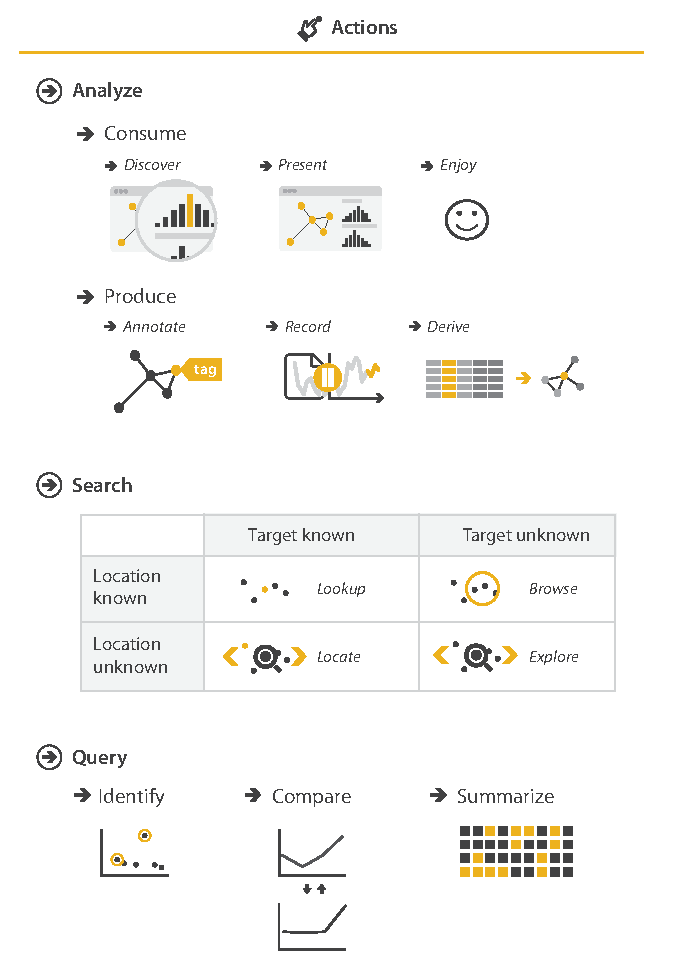
\includegraphics[width=0.85\textwidth]{figures/fig3-2.pdf}
    \caption
    [
        The \textsl{why} part of our typology, slightly extended and recast as a set of \textsl{actions}.
    ]
    {
        The \textsl{why} part of our typology, slightly extended as per \autoref{drvistasks:typology} and recast as a set of {\tt actions}~\cite{Munzner2014}; \cf \autoref{typology:fig:typology}a. Illustration: \ccLogo~E. Maguire (2014).
    }
	\centering
	\label{fig:typology-actions}
\end{figure}

%-|-|-|-|-|-|-|-|-|-|-|-|-|-|-|-|-|-|-|-|-|-|-|-|-|-|-|-|-|-|-|-|-|-|-|-|-

%-|-|-|-|-|-|-|-|-|-|-|-|-|-|-|-|-|-|-|-|-|-|-|-|-|-|-|-|-|-|-|-|-|-|-|-|-

\begin{figure}
	\centering
    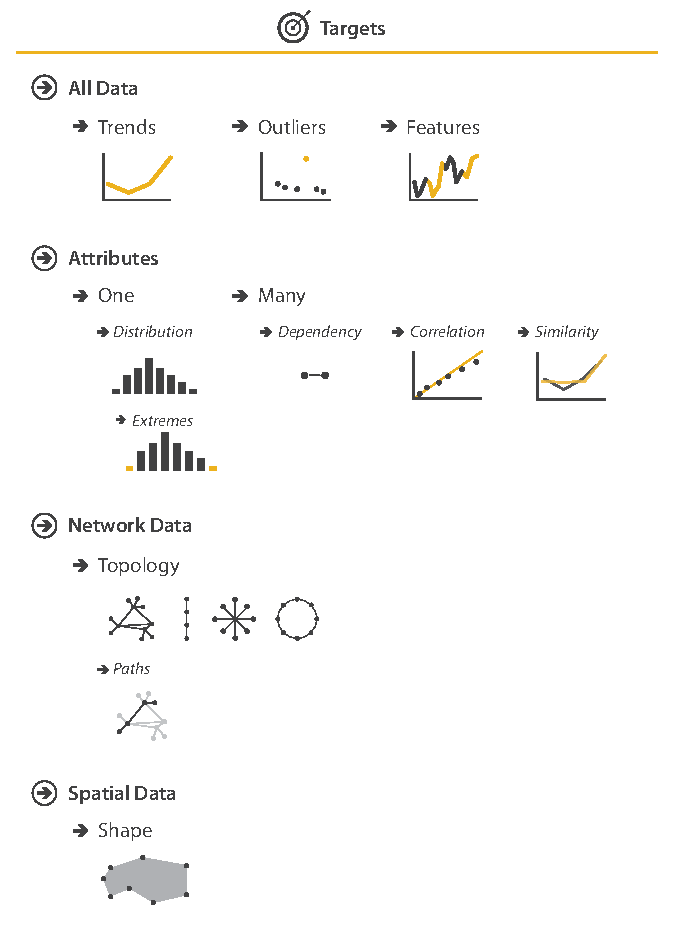
\includegraphics[width=0.85\textwidth]{figures/fig3-6.pdf}
    \caption
    [
        A set of \underline{{\tt targets}}, to be used in conjunction with a specification of {\tt actions}.
    ]
    {
       A set of \underline{{\tt targets}}, to be used in conjunction with a specification of {\tt actions} drawn from the set in \autoref{fig:typology-actions}~\cite{Munzner2014}. Illustration: \ccLogo~E. Maguire (2014).
    }
	\centering
	\label{fig:typology-targets}
\end{figure}

%-|-|-|-|-|-|-|-|-|-|-|-|-|-|-|-|-|-|-|-|-|-|-|-|-|-|-|-|-|-|-|-|-|-|-|-|-

\citet{Munzner2014} has also introduced a classification of {\it what}\index{{\tt what}}, shown in \autoref{fig:typology-vad-what}, a remarkable difference from our ``bring your own {\it what}\index{{\tt what}}'' mentality discussed in \autoref{typology:what}, where we suggested that a simple specification {\tt inputs}\index{{\tt input}} and {\tt outputs}\index{{\tt output}} was sufficient for describing tasks\index{task} and task sequences\index{task!task sequence}.
Munzner's classification of {\it what}\index{{\tt what}} refers to abstract datatypes, attribute types, and dataset availability, among other criteria.

%-|-|-|-|-|-|-|-|-|-|-|-|-|-|-|-|-|-|-|-|-|-|-|-|-|-|-|-|-|-|-|-|-|-|-|-|-

\begin{figure}
	\centering
    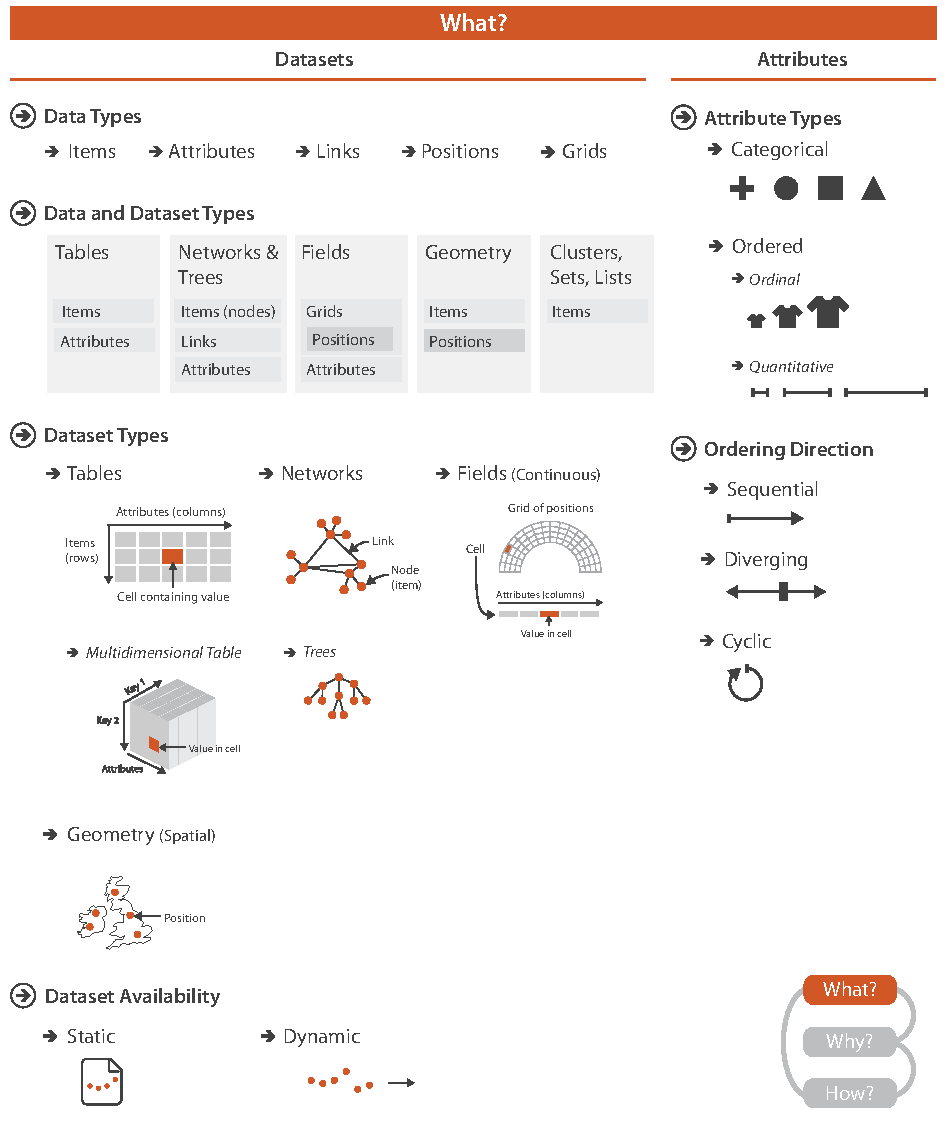
\includegraphics[width=\textwidth]{figures/fig2-1.pdf}
    \caption
    [
        Munzner's classifcation of \textsl{what}~\cite{Munzner2014}.
    ]
    {
        Munzner's classifcation of \textsl{what}~\cite{Munzner2014}. Illustration: \ccLogo~E. Maguire (2014).
    }
	\centering
	\label{fig:typology-vad-what}
\end{figure}

%-|-|-|-|-|-|-|-|-|-|-|-|-|-|-|-|-|-|-|-|-|-|-|-|-|-|-|-|-|-|-|-|-|-|-|-|-

Finally, \citet{Munzner2014} has proposed a revision to the {\it how}\index{{\tt how}} part of the typology\index{task!task typology}, as indicated by \autoref{fig:typology-vad-how}. 
Relative to our original formulation of the typology\index{task!task typology} (\cf \autoref{typology:fig:typology}b), Munzner expands upon subtypes of {\tt encode}\index{{\tt encode}} and further distinguishes between {\tt manipulate}\index{{\tt manipulate}} (retaining subtypes {\tt navigate}\index{{\tt navigate}}, {\tt select}\index{{\tt select}}, and {\tt change}\index{{\tt change}}), {\tt facet}\index{view coordination!faceting (small multiples)} (formerly {\tt arrange}\index{{\tt arrange}}, now with subtypes {\tt juxtapose}\index{view coordination!view juxtaposition}, {\tt superimpose}, and {\tt partition}), and {\tt reduce} (encompassing {\tt filter}\index{{\tt filter}} and {\tt aggregate}\index{{\tt aggregate}}, along with the previously absent {\tt embed}).
% We adopted this extension to {\it how}\index{{\tt how}} in the addendum to \autoref{ch:emu} (see \autoref{emu:addendum}).

%-|-|-|-|-|-|-|-|-|-|-|-|-|-|-|-|-|-|-|-|-|-|-|-|-|-|-|-|-|-|-|-|-|-|-|-|-

\begin{figure}
	\centering
    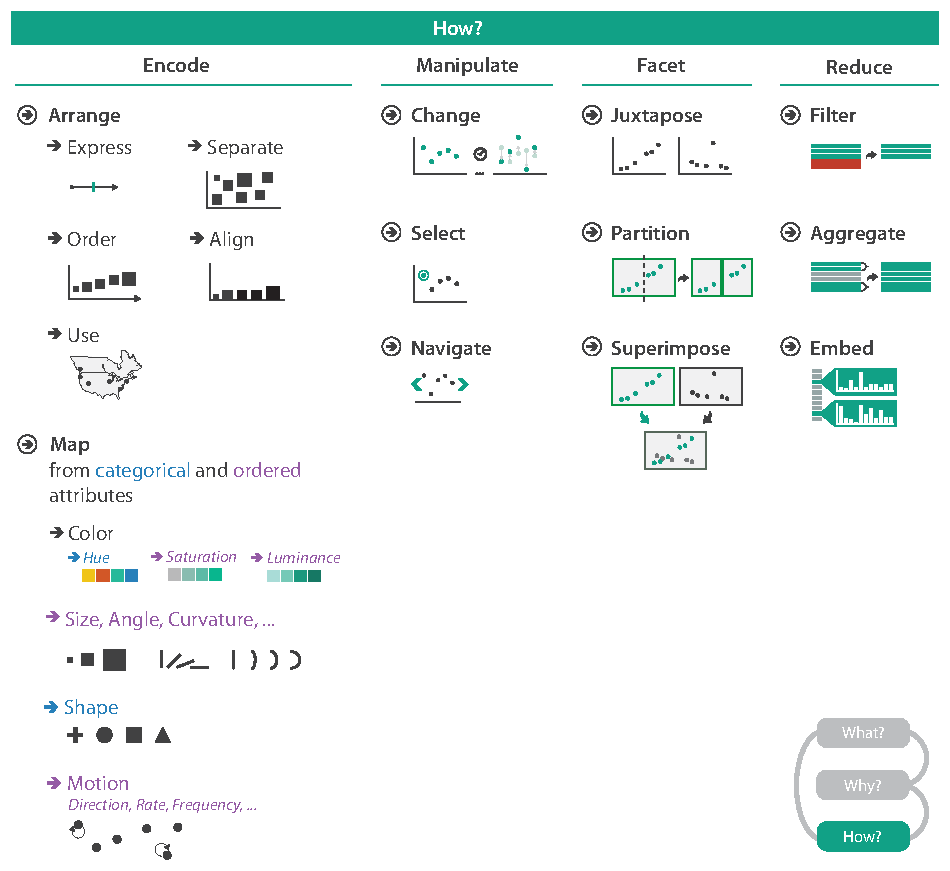
\includegraphics[width=\textwidth]{figures/fig3-7.pdf}
    \caption
    [
        Munzner's extension~\cite{Munzner2014} to the \textsl{how} part of our typology.
    ]
    {
        Munzner's extension~\cite{Munzner2014} to the \textsl{how} part of our typology; \cf \autoref{typology:fig:typology}b. Illustration: \ccLogo~E. Maguire (2014).
    }
	\centering
	\label{fig:typology-vad-how}
\end{figure}

%-|-|-|-|-|-|-|-|-|-|-|-|-|-|-|-|-|-|-|-|-|-|-|-|-|-|-|-|-|-|-|-|-|-|-|-|-

\bstart{Commentary on these extensions}
Our typology\index{task!task typology} of visualization tasks\index{task} is an evolving entity, a proposal that the visualization community might use to classify tasks, and Munzner's extensions are part of this evolution, along with the efforts of other researchers who have extended our typology to speak about tasks involving specific datatypes or domains, which we discuss below in \autoref{conclusions:typology:adoption}.

Is this variability and evolution a problem? 
Not necessarily. 
One the one hand, Munzner's proposed modifications allow us to create more specific descriptions of {\it how}\index{{\tt how}} a visualization technique or tool can support a task\index{task}, as well as {\it what} these tasks pertain to.
We surely benefited from Munzner's modifications in our interview study (\autoref{ch:drvistasks}) and in our design study (\autoref{ch:emu}), in which we acknowledged the {\tt introduce}\index{{\tt introduce}} nodes being reclassified as forms of {\tt produce}\index{{\tt produce}} and the addition of \underline{{\tt targets}}\index{{\tt targets}}, respectively.
On the other hand, an evolving classification is more difficult to learn, and may complicate communication between researchers, practitioners, and students, which surely reduces the benefit of having a common lexicon for describing tasks. 
Furthermore, one could argue that with the increase in specificity that Munzner's modifications bring, there is a reduction in flexibility. 
For instance, by leaving {\tt input}\index{{\tt input}}, {\tt output}\index{{\tt output}}, and {\tt encode}\index{{\tt encode}} as open-ended placeholder terms in our original typology, people were free to consider inputs and outputs specific to their situation, or whichever visual encoding\index{visual encoding} they could imagine.

Munzner's decision to move {\tt introduce}\index{{\tt introduce}} nodes {\tt annotate}\index{{\tt annotate}}, {\tt record}\index{{\tt record}}, and {\tt derive}\index{{\tt derive}} from the {\it how}\index{{\tt how}} part of our typology\index{task!task typology} to the {\it why}\index{{\tt why}} part of our typology\index{task!task typology} as subtypes of {\tt produce}\index{{\tt produce}} reflects an uncertainty about these terms that appeared throughout the typology's history (see \autoref{app:typology}): at one point, {\tt derive}\index{{\tt derive}} was classified under the question of {\it which} (see \autoref{app:typology:fig:13.01.09}); earlier, {\tt annotate}\index{{\tt annotate}} and {\tt record}\index{{\tt record}} were classified as {\it provenance tasks} along with {\tt present}\index{{\tt present}} (see \autoref{app:typology:fig:12.11.23}).
This uncertainty with regards to whether {\tt annotate}\index{{\tt annotate}}, {\tt record}\index{{\tt record}}, and {\tt derive}\index{{\tt derive}} fit best under {\it why}\index{{\tt why}} or {\it how}\index{{\tt how}} seems to imply that they could be seen as either ends\index{task!ends} or means\index{task!means}, subject to context and their position within a sequence of tasks\index{task!task sequence}. 
For now, the advantage of thinking of {\tt annotate}\index{{\tt annotate}}, {\tt record}\index{{\tt record}}, and {\tt derive}\index{{\tt derive}} as forms of {\tt produce}\index{{\tt produce}} in the {\it why}\index{{\tt why}} part of our typology\index{task!task typology} is that it forces us to consider {\it how}\index{{\tt how}} the annotation, recording, or derivation are supported by a visualization tool.
For instance, consider {\tt annotate}\index{{\tt annotate}}: annotation may be supported with {\tt selection}\index{{\tt select}} of visualized data elements via direct manipulation, or an automatic annotation of data elements may occur in response to interactive {\tt navigation}\index{{\tt navigate}} or {\tt aggregation}\index{{\tt aggregate}}.

Munzner's addition of \underline{{\tt targets}}\index{{\tt targets}} and a thorough classification of {\it what}\index{{\tt what}} is also not surprising given the history of our typology\index{task!task typology}.
In \autoref{app:typology}, we document how earlier drafts of what would be become our typology\index{task!task typology} included a classification of {\it what}\index{{\tt what}} beyond {\tt input}\index{{\tt input}} and {\tt output}\index{{\tt output}}\footnote{See Figures~\ref{app:typology:fig:12.12.09}~--~\ref{app:typology:fig:13.02.25}.}.
We realized that we could not present a satisfyingly comprehensive classification of {\it why}\index{{\tt why}}, {\it how}\index{{\tt how}}, and {\it what}\index{{\tt what}} in a single 10-page paper submission to IEEE InfoVis, and thus we opted to focus on {\it why}\index{{\tt why}} and {\it how}\index{{\tt how}}.
Nevertheless, I personally prefer the flexibility that comes with thinking about {\it what}\index{{\tt what}} simply in terms of {\tt input}\index{{\tt input}} and {\tt output}\index{{\tt output}}, as this line of thinking also primes one to think in terms of task sequences\index{task!task sequence} and interdependencies, while there is no explicit sequence-based language in Munzner's \underline{{\tt targets}}\index{{\tt targets}} or in her classification of {\it what}\index{{\tt what}}.
Furthermore, I view Munzner's \underline{{\tt targets}}\index{{\tt targets}} and her classification of {\it what}\index{{\tt what}} as suggestions, like any term in our original typology: if a person has more specific terms in mind, she should be encouraged to use them in place of our abstract conceptual terms, especially if it helps her to think.
This reflects how others have used our typology, which we describe below in \autoref{conclusions:typology:adoption}: they retain the {\it why-what-how} structure of our typology and perhaps some of our vocabulary, while introducing their own terms to create new a datatype or domain specific taxonomy.
In summary, out typology\index{task!task typology} is part of an ongoing conversation about tasks, and any incarnation of it should not be interpreted as a rigid system.

%-------------------------------------------------------------------------

\subsection{Comparisons to Roth (2013), Schulz~\etal~(2013)}
\label{conclusions:typology:contemporary}

%-------------------------------------------------------------------------

When I presented our typology\index{task!task typology} paper~\cite{Brehmer2013} at IEEE InfoVis 2013, my presentation was preceded by a classification of interaction\index{interaction} primitives for cartographic\index{cartography} data by \citet{Roth2013} (an extension of his 2012 {\it GIScience} workshop paper~\cite{Roth2012}, which we included in the literature review that grounded our typology\index{task!task typology}).
My presentation was also preceded by ``{\it A Design Space of Visualization Tasks}'' by \citet{Schulz2013}, which independently arrived at some of the same defining questions forming the structure our typology\index{task!task typology}, namely {\it why}\index{{\tt why}} a task pursued (the {\it goal} of the task), {\it how}\index{{\tt how}} a task is carried out (the {\it means} of the task), and {\it what}\index{{\tt what}} a task seeks (the data {\it characteristics}); they also pose the questions of {\it where} does a task\index{task} operate in the data (the {\it target} and {\it cardinality} of data entities within that target), {\it when} a task\index{task} is performed (for specifying the order of tasks), and {\it who} is executing the task\index{task} (for specifying the type of user). \citet{Schulz2013} further introduce a formal notation for describing tasks\index{task}, and they realize their design space with an implementation of a tool for recommending visualization techniques in relation to climate impact data.

There are certainly ideas that are common between our typology\index{task!task typology} and the classifications of \citet{Roth2013} and \citet{Schulz2013}, however there are also notable differences: there are aspects of tasks that we account for that these other classifications do not (and vice versa), as well as aspects that we organize in a different way.
Moreover, if we consider the external influences on these three classifications in terms of their bibliographies, only seven references are shared by all three papers\footnote{\citet{Amar2005,Chuah1996,Pirolli2005,Shneiderman1996,Wehrend1990,Yi2007,Zhou1998}. We also have 12 references in common with both \citet{Roth2013} and \citet{Schulz2013}, who in turn share 8 common references that we do not cite.}.

At the highest level, the three questions of our typology\index{task!task typology} suggests a correspondence with the dimensions of Schulz and colleagues' design space~\cite{Schulz2013} and with the four parts of Roth's taxonomy~\cite{Roth2013}.

One might expect that our question of {\it why}\index{{\tt why}} a task is undertaken to overlap with Roth and Schulz~\etal's characterization of {\it goals}, however we also observed a partial overlap with the design space's dimensions of {\it means} and {\it cardinality}, as well as with Roth's {\it objectives} and {\it operators}.
Schulz and colleagues have analogues to {\tt present}\index{{\tt present}} and {\tt discover}\index{{\tt discover}}, and our definition of {\tt discover}\index{{\tt discover}} similarly refers to the {\it generating}, {\it refining}, and {\it verifying} of hypotheses.
Meanwhile, Roth's {\it procure} bears a similarity to our definition of {\tt consume}\index{{\tt consume}}; while his {\it predict} and {\it prescribe} suggest an even higher-level motivation for {\tt consuming}\index{{\tt consume}} information, as {\it predict} and {\it prescribe} are often associated with decision making processes.
We are unique in that we include the term {\tt produce}\index{{\tt produce}}, the converse of {\tt consume}\index{{\tt consume}}, which allows us to account for tasks that {\tt produce}\index{{\tt produce}} new information.
Moving further down the {\it why}\index{{\tt why}} part of our typology\index{task!task typology}, we claim a unique characterization of {\tt search}\index{{\tt search}} that depends on whether the identify and location of the search target are known a priori. 
Our characterization of {\tt search}\index{{\tt search}} overlaps somewhat with Schulz and colleagues' {\it goals} pertaining to {\it directed} and {\it undirected search}; it also relates to their definition of {\it navigation}, listed as a {\it means} in their design space. 
Our characterization of {\tt search}\index{{\tt search}} also differs from that of Roth's taxonomy, which includes several related {\tt search}\index{{\tt search}} terms but defined as {\it operators}. 
With regards to our {\tt query}\index{{\tt query}} types: {\tt identify}\index{{\tt identify}}, {\tt compare}\index{{\tt compare}}, and {\tt summarize}\index{{\tt summarize}}, there is an obvious mapping to the {\it cardinality} dimension of Schulz~\etal's design space, which refers to {\it single instances}, {\it multiple instances}, and {\it all instances} of available data; meanwhile, our {\tt query} types would be {\it objectives} according to Roth, which increase in sophistication along with {\it cardinality}.

Our question of {\it how}\index{{\tt how}} a task is supported has a clearer correspondence to both Schulz~\etal's {\it means} and Roth's {\it operators}; in particular, how we distinguish {\tt manipulate}\index{{\tt manipulate}} and {\tt introduce}\index{{\tt introduce}}\footnote{{\tt introduce} nodes became forms of {\tt produce} in Munzner's extension to the typology~\cite{Munzner2014}.} partially corresponds with Roth's distinction between {\it enabling operators} and {\it work operators}.
Nevertheless, there are still a number of subtle differences worth pointing out.
For one, we include {\tt encode}\index{{\tt encode}}, which relates directly to how the data is visually encoded\index{visual encoding}. 
Based on the absence or presence of other methods in a task description, we can discern between static and interactive visualization artefacts.
Another term unique to our typology\index{task!task typology} is {\tt change}\index{{\tt change}}, a verb which might appear vague without a qualifying noun; this term is found in many previous classifications, perhaps pertaining to a change in visual encoding\index{visual encoding} parameters, scale, or an animated transformation\index{view coordination!animated transitions}. 
When used in the context of a full task description that includes explicitly defined {\tt inputs}\index{{\tt input}} and {\tt outputs}\index{{\tt output}}, the meaning of {\tt change}\index{{\tt change}} is no longer unclear.

Another prominent difference from our typology\index{task!task typology} and the classifications of \citet{Roth2013} and \citet{Schulz2013} is in our handling of {\it what}\index{{\tt what}}.
Our characterization of {\it what}\index{{\tt what}}, comprising of a task's {\tt inputs}\index{{\tt input}} and {\tt outputs}\index{{\tt output}}, overlaps partially with several dimensions of the Schulz~\etal's design space, as well as with Roth's {\it operands}.
In early drafts, we tried to classify {\it what}\index{{\tt what}} comprises a visualization in more detail (documented throughout \autoref{app:typology}), but our classification became far too complicated, and we decided to talk about {\it what} in greater detail in \citet{Munzner2014}\footnote{Summarized in \autoref{fig:typology-vad-what}, above; it is also worth noting that \citet{Munzner2014} also uses the term \underline{{\tt targets}}, a term used by \citet{Schulz2013}.}.
We simplified to the agnostic ``bring your own {\it what}\index{{\tt what}}'' mentality discussed in \autoref{typology:what}, as we realized that as long as one specifies the {\tt inputs}\index{{\tt input}} and {\tt outputs}\index{{\tt output}} of a task, any classification of visualization elements can be used, including the {\it operand} classification by \citet{Roth2013} or the {\it characteristics} and {\it target} classifications by \citet{Schulz2013}.

Yet another difference is that \citet{Roth2013} and \citet{Schulz2013} do not explicitly accommodate the casual use of visualization artefacts, this being usage motivated not by a need to {\tt present}\index{{\tt present}} or {\tt discover}\index{{\tt discover}} information, whereas we use the term {\tt enjoy}\index{{\tt enjoy}} to describe such tasks.

A final difference to illustrate, particularly between our typology\index{task!task typology} and the classification by \citet{Schulz2013}, is how these classifications can be used to describe task sequences\index{task!task sequence}.
\citet{Schulz2013} provide a textual notation for describing what they refer to as workflows\index{workflows}, and they offer an example in their paper where they use their ({\it goals, means, characteristics, target, cardinality}) notation to describe the Shneiderman's well-known {\it visual information seeking mantra}~\cite{Shneiderman1996}\index{visual information seeking mantra (Shneiderman)}: {\it overview first, zoom \& filter, details-on-demand}\index{view coordination!details-on-demand}:

\begin{quotation}
    % \bstart{overview}
    ({\it exploratory}, {\it summarize}, \textasteriskcentered, \textasteriskcentered, {\it all}) $\Rightarrow$
    
    % \bstart{zoom \& filter}
    ({\it exploratory}, {\it elaborate} \textbar~{\it filter}, \textasteriskcentered, \textasteriskcentered, {\it multiple}) $\Rightarrow$
    
    % \bstart{details-on-demand}
    ({\it exploratory} \textbar {\it confirmatory}, {\it gather} \textbar~{\it look-up}, \textasteriskcentered, {\it single})
\end{quotation}

Our corresponding visual notation, shown in \autoref{fig:typology-mantra}, captures the same three steps while explicitly indicating the links between {\tt inputs}\index{{\tt input}} and {\tt outputs}\index{{\tt output}} of subsequent tasks in the sequence.
In the {\it overview first} task, a person {\tt explores}\index{{\tt explore}} and {\tt summarizes}\index{{\tt summarize}} an {\it overview of the data}, which is supported by the visual {\tt encoding}\index{{\tt encode}}\index{visual encoding}.
In the {\it zoom \& filter} step, she {\tt browses}\index{{\tt browse}} the {\it overview} to {\tt identify}\index{{\tt identify}} a {\it subset of items} that interests her, supported by {\tt navigation}\index{{\tt navigate}} and {\tt filtering}\index{{\tt filter}}.
Finally, in the {\it details-on-demand} step, she {\tt browses}\index{{\tt browse}} that {\it subset} and {\tt identifies}\index{{\tt identify}} a particular item that interests her, {\tt navigating}\index{{\tt navigate}} and {\tt selecting}\index{{\tt select}} it to learn more.
Also note that each part of the {\it overview first, zoom \& filter, details-on-demand} mantra\index{visual information seeking mantra (Shneiderman)} is about {\tt consuming} information, and it could apply equally to {\tt present}\index{{\tt present}}, {\tt discover}\index{{\tt discover}}, or {\tt enjoy}\index{{\tt enjoy}} contexts. 

%-|-|-|-|-|-|-|-|-|-|-|-|-|-|-|-|-|-|-|-|-|-|-|-|-|-|-|-|-|-|-|-|-|-|-|-|-

\begin{figure}[ht!]
	\centering
    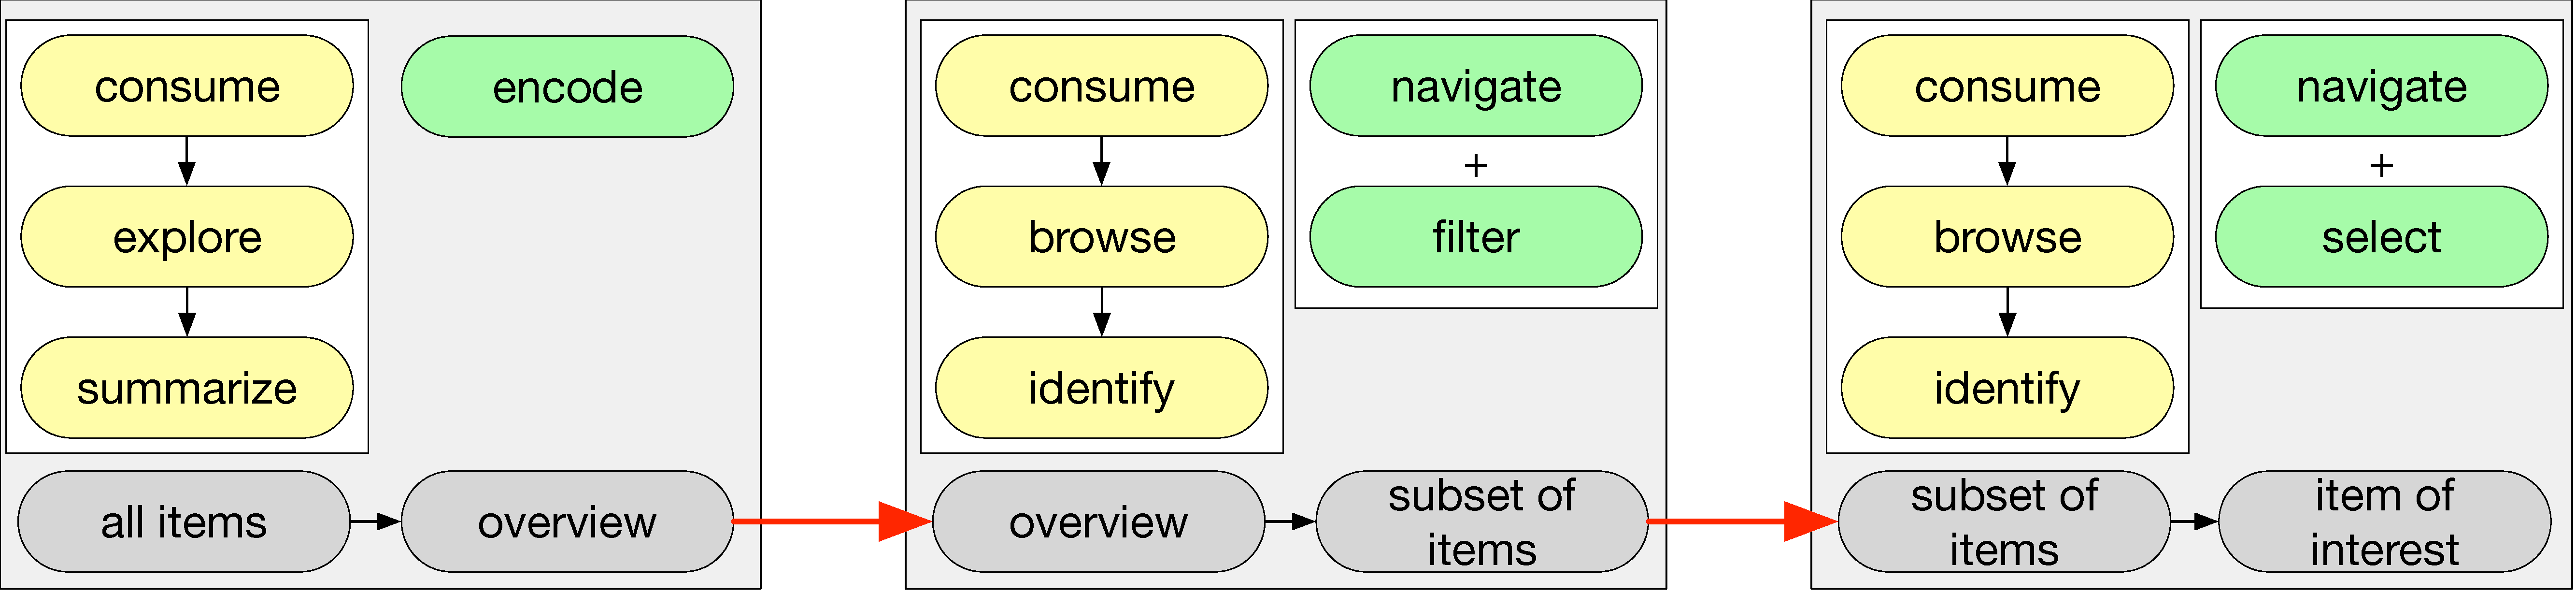
\includegraphics[width=\textwidth]{figures/typology-mantra.pdf}
    \caption
    [
        Our typology is used to describe Shneiderman's {\it visual information seeking mantra}: {\it overview first, zoom and filter, details-on-demand}.
    ]
    {
        Our typology is used to describe Shneiderman's {\it visual information seeking mantra}: {\it overview first, zoom \& filter, details-on-demand}.
    }
	\centering
	\label{fig:typology-mantra}
\end{figure}

%-|-|-|-|-|-|-|-|-|-|-|-|-|-|-|-|-|-|-|-|-|-|-|-|-|-|-|-|-|-|-|-|-|-|-|-|-

%-------------------------------------------------------------------------

\subsection{Impact of the Task Typology}
\label{conclusions:typology:adoption}

%-------------------------------------------------------------------------

In addition to playing an important role in the three other projects described in \autoref{ch:drvistasks},~\ref{ch:overview}, and~\ref{ch:emu}, our task typology has had considerable impact within the visualization community.
Our task typology\index{task!task typology} paper~\cite{Brehmer2013} has been cited over 60 times\footnote{According to Google Scholar, excluding self-citations, as of \today.}, and it is one of the most-cited papers from IEEE {\it Transactions on Visualization and Computer Graphics} published since Fall 2013 (Volume 19, Number 12, Proceedings of InfoVis 2013).

Papers written by other researchers which cite our typology\index{task!task typology} paper include eight IEEE {\it Transactions on Visualization and Computer Graphics} journal papers~\cite{Blascheck2015,Kerracher2015,Kindlmann2014,Sacha2014,Saket2014,Scheepens2015,Sedlmair2014,Zhou2015}\footnote{According to Google Scholar, IEEE {\it TVCG} papers have the second highest impact factor in the field of computer graphics, following ACM {\it Transactions on Graphics}.}, an IEEE {\it Symposium on Visual Analytics Science and Technology (VAST)} paper~\cite{Gomez2014}, three {\it Computer Graphics Forum (Proceedings of EuroVis)} journal papers~\cite{Conati2014,Saket2015,Walny2015}, four {\it EuroVis Short Papers}~\cite{Mittelstadt2015,Nusrat2015,Saket2014a,Saket2015a}, two {\it EuroVis State of the Art Reports}~\cite{Blascheck2014,Wagner2015}, three {\it Information Visualization} journal articles~\cite{Rind2015,Simon2015,Winters2015}, and an ACM {\it Human Factors in Computing Systems (CHI)} conference paper~\cite{Taher2015}.
Our typology\index{task!task typology} paper has also been cited in papers presented at various other conferences, symposia, and workshops, as well as in a number of journal articles, technical reports, and theses.
In addition to informing the work of other researchers, we have also referred to our task typology in other subsequent papers appearing in IEEE {\it Transactions on Visualization and Computer Graphics}~\cite{Fulda2015}, the {\it Information Visualization} journal~\cite{Dawson2015,Meyer2015}, and at the ACM BELIV workshop~\cite{Brehmer2014a}. 

Other researchers have discussed the typology\index{task!task typology} in the context of new models or frameworks.
In the {\it knowledge generation model for visual analytics}\index{visual analytics} by \citet{Sacha2014}, our typology\index{task!task typology} is invoked in relation to their discussion of a {\it exploration loop} and a {\it verification loop}, wherein lower-level actions are associated with the former and higher-level actions are associated with the latter. 
Meanwhile, in the {\it algebraic process for visualization design} by \citet{Kindlmann2014}, the concept of {\it data symmetries}, or transformations in data space, are associated with the {\tt manipulate}\index{{\tt manipulate}} nodes in the {\it how}\index{{\tt how}} part of our typology\index{task!task typology}.
\citet{Rind2015} discuss our typology\index{task!task typology} (among many other classifications of tasks) in the context of their meta-analysis of task\index{task} classifications, defining three dimensions for describing the space of task\index{task} classifications: {\it abstraction} (concrete vs. abstract)\index{task!task abstraction}, {\it composition} (high-level vs. low-level), and {\it perspective} ({\it why} vs. {\it how}).
Finally, in a conceptual model for characterizing domain problems by \citet{Winters2015}, they describe different types of people who use visualization tools, and how these people are typically either those that {\tt produce}\index{{\tt produce}} information or those that {\tt consume}\index{{\tt consume}} information.

There are several new task\index{task} classifications specific to particular datatypes that adopt the vocabulary and/or the {\it why-what-how}\index{{\tt why}}\index{{\tt what}}\index{{\tt how}} structure of our typology\index{task!task typology}, including those relating to node-link-group data~\cite{Saket2014,Saket2014a}\index{network data}, cartograms~\cite{Nusrat2015}, multiplex networks~\cite{Renoust2013}\index{network data}, and multidimensional data projections~\cite{Etemadpour2015}\index{dimensionality reduction (DR)}.
Other novel datatype-specific classifications that refer to our typology\index{task!task typology} include classifications of tasks\index{task} for multivariate network analysis~\cite{Pretorius2014}\index{network data} and temporal graphs~\cite{Kerracher2015}\index{network data}\index{time-oriented data}; while these classifications do not adopt our typology's\index{task!task typology} vocabulary or structure, their authors reiterate our arguments about the purpose of classifying visualization tasks\index{task}, and \citet{Kerracher2015} they explicitly motivate their work in response to our call for more datatype-specific classification of tasks\index{task} (see \autoref{typology:rw:taxonomies}).

\begin{sloppypar}
There are also several application-domain specific classifications of tasks\index{task} that adopt or extend our typology\index{task!task typology}, again using our vocabulary and/or the {\it why-what-how}\index{{\tt why}}\index{{\tt what}}\index{{\tt how}} structure, including those specific to bioinformatics\index{bioinformatics}~\cite{Mirel2014}, computational chemistry~\cite{Vanderwoning2014}\index{chemistry}, telemedicine~\cite{Theisa2015}, and malware analysis~\cite{Wagner2015}.
One particularly unusual and fascinating adoption of our typology\index{task!task typology} is a classification of tasks\index{task} related to artistic human plant interfaces~\cite{Weil2014}.
\end{sloppypar}

Applying our typology\index{task!task typology} to a specific domain or datatype is not always a straightforward endeavour, as indicated by \citet{Sedlmair2014} in their classification of visual parameter space analysis tasks\index{task}:

\begin{quote}

    {\it ``While we found the general categories of why and how helpful in guiding our analysis, we could not directly match our framework into this typology\index{task!task typology}. Our work addresses analysis tasks\index{task} specific to visual parameter space analysis that have not been discussed in their typology.''}~\citep[p. 2167]{Sedlmair2014}
    
\end{quote}

\citet{Sedlmair2014} reiterate our call for additional datatype-specific and domain-specific classifications of tasks\index{task}, and they ultimately characterize six tasks\index{task}: {\it optimization}, {\it partitioning}, {\it fitting}, {\it outliers}, {\it uncertainty}\index{uncertainty}, and {\it sensitivity}\index{sensitivity analysis}. 
It would be an interesting exercise to express these six tasks\index{task} using the vocabulary and structure of our typology\index{task!task typology}, tasks\index{task} which are highly intertwined with other data analysis and simulation activities beyond those that directly involve a visual encoding\index{visual encoding}.

Others have used our typology\index{task!task typology} in specifying the tasks\index{task} addressed by novel visualization techniques or tools, such as in a technique for analyzing traffic flows~\cite{Scheepens2015}, in the design of a multi-touch tangible user interface for biological data visualization~\cite{Almegren2016}, in ColorCAT, a colour map creation tool~\cite{Mittelstadt2015}, or in VA$^2$, a tool for evaluating\index{evaluation} the eye movements and interactions\index{interaction} of people while using visual analytics\index{visual analytics} tools~\cite{Blascheck2015}.
Our typology\index{task!task typology} has also been used to describe the capabilities of a family of off-screen visualization techniques~\cite{Jackle2015}.
We also note the use of our typology\index{task!task typology} to characterize the tasks\index{task} addressed by VisExpress, a recent design study\index{design studies} project in the bioinformatics\index{bioinformatics} domain~\cite{Simon2015}.

Finally, 
% \citet{Conati2014} used our typology\index{task!task typology} used as a basis for motivating the tasks in experimental work on individual differences and interface layout, while 
\citet{Saket2015} have used our typology\index{task!task typology} to specify tasks\index{task} in an experiment comparing map-based and node-link graph\index{visual encoding!node-link graph} layouts.

Altogether, we are very pleased with how our typology\index{task!task typology} has been adopted.
In \autoref{typology:discussion}, we proposed ways in which our typology\index{task!task typology} could be used to {\it describe} (or {\it analyze}) the use of visualization tools or techniques, {\it evaluate}\index{evaluation} these tools or techniques, and {\it generate} new designs; this brief survey has revealed that the typology\index{task!task typology} has accomplished all of these goals: it has described the use of visualization tools and techniques in the context of specific domains or datatypes, it has been used in the specification of tasks\index{task} for experimental evaluation\index{evaluation} studies, and it has grounded the design of new visualization tools and techniques.

We also note the variability with respect to how aspects of our typology\index{task!task typology} have been used.
While some adopt the {\it why-what-how}\index{{\tt why}}\index{{\tt what}}\index{{\tt how}} framing, others use specific vocabulary from parts of our typology\index{task!task typology}, while some have even adopted the visual style of our task\index{task} diagrams, such as those used in \autoref{ch:typology} (\eg ~\cite{Jackle2015,Vanderwoning2014}).
This variability is not surprising; we did not imagine or intend that our typology\index{task!task typology} would be used to develop a rigid specification of tasks\index{task}; we reiterate that it our typology\index{task!task typology} is a proposal of how to classify tasks: it is not the final answer, and we invite others to extend it and propose alternatives.
Our own use of the typology\index{task!task typology} has also varied and evolved between \autoref{ch:drvistasks}, \autoref{ch:overview}, and \autoref{ch:emu}, especially since the advent of Munzner's extension to the typology~\cite{Munzner2014}\index{task!task typology}, and we expect that our use of the typology\index{task!task typology} will continue to evolve in our future projects.

\bstart{Other uses of the typology}
In addition to its adoption and extension by the visualization research community, the typology\index{task!task typology} has also appeared in other contexts.

For instance, our typology\index{task!task typology} was featured in a 2014 IEEE VIS conference tutorial by \citet{McNamara2014} on practical methods for design studies\index{design studies}, where our typology\index{task!task typology} was referred to as a viable tool for task abstraction\index{task!task abstraction} following the work domain analysis\index{work domain analysis} phase of a design study\index{design studies} project.

Another interesting use of the typology\index{task!task typology} was in an interactive faceted browser by \citet{Yalcin2014}, in which he visualized the vocabulary and bibliography of our typology\index{task!task typology} paper\footnote{\url{http://keshif.me/demo/vis_tasks.html}}.

Our typology\index{task!task typology} paper~\cite{Brehmer2013} has also been included on the syllabi of several graduate courses in visualization\footnote{These include courses taught at the University of Chicago (\url{http://goo.gl/htBFju}), the University of Utah (\url{http://goo.gl/cLsJmY}), the University of Wisconsin-Madison (\url{http://goo.gl/lsRAHC}), Tufts University, and at the University of British Columbia (\url{http://goo.gl/Xt7ry2})}; many visualization courses are also making use of Munzner's book~\cite{Munzner2014}, and thus are reading about our typology\index{task!task typology} indirectly\footnote{A list of these courses can be found here: \url{http://cs.ubc.ca/~tmm/vadbook/}}.
Our paper is also listed on the computer science doctoral qualifying resources list for students pursuing research in information visualization at Georgia Tech\footnote{\url{http://goo.gl/GY3hQw}}.
These institutions are well-known for visualization research, and it is encouraging to see that our typology\index{task!task typology} is reaching the next generation of researchers and practitioners.

%-------------------------------------------------------------------------
%-------------------------------------------------------------------------

\section{Reflecting on the Interview Study}
\label{conclusions:drvistasks}

%-------------------------------------------------------------------------
%-------------------------------------------------------------------------

The study reported in \autoref{ch:drvistasks} was preceded by a technical report entitled {\it Dimensionality Reduction in the Wild: Gaps and Guidance}~\cite{Sedlmair2012b}; in addition to informing our own subsequent work~\cite{Hammer2015,Ingram2013,Ingram2015,Sedlmair2013,Sedlmair2014}, the paper and technical report have garnered over fifteen citations by others in the visualization community\footnote{According to Google Scholar (as of \today)}.

Like our original task typology in \autoref{ch:typology}\index{task!task typology}, our classification of task sequences\index{task!task sequence} relating to dimensionally reduced\index{dimensionality reduction (DR)} data can also be discussed in relation to subsequent work.
One of the papers mentioned above that extends and refers to the {\it why-what-how}\index{{\tt why}}\index{{\tt what}}\index{{\tt how}} structure of our original typology\index{task!task typology} is a datatype specific classification of tasks\index{task} by \citet{Etemadpour2015}, one specific to multidimensional data projections (in other words, visual encodings\index{visual encoding} of dimensionally reduced\index{dimensionality reduction (DR)} data).
\citet{Etemadpour2015} consolidate all of the tasks\index{task} that are explicitly or implicitly addressed in previous \ac{DR}\index{dimensionality reduction (DR)} technique papers. 
They arrive at a classification of four groups of tasks\index{task} (35 tasks in total): 
seven {\it pattern identification}\index{{\tt identify}} tasks\index{task}, fourteen {\it relation-seeking} tasks, ten {\it behaviour comparison} tasks\index{task}, and four {\it membership disambiguation} tasks\index{task}. 
The individual tasks are quite specific and are worded much like instructions in a controlled experiment, such as {\it estimate the number of observed clusters} (a {\it pattern identification}\index{{\tt identify}} task), or {\it find the cluster with the most/least number of points or size} (a {\it behaviour comparison} task).
Though they do not define each of the 35 tasks\index{task} in detail, they do provide two examples in which they decompose the task\index{task} using our typology's\index{task!task typology} vocabulary and {\it why-what-how}\index{{\tt why}}\index{{\tt what}}\index{{\tt how}} structure.

Recall that in \autoref{ch:drvistasks}, we characterized five task\index{task} sequences\index{task!task sequence} relating to the visualization of dimensionally reduced\index{dimensionality reduction (DR)} data: two focused on dimensions ({\it name synthetic dimensions} and {\it map synthetic dimensions to original dimensions}), while three focused on clusters ({\it verifying that clusters exist}, {\it naming clusters}, and {\it matching clusters and classes}). 
In contrast, the list of 35 tasks\index{task} by \citet{Etemadpour2015} pertains almost exclusively to clusters and their spatial or quantitative properties (30 tasks), while the remaining five tasks\index{task} focus on individual points or outliers; there are no tasks\index{task} pertaining to {\it naming the projected synthetic dimensions} or {\it understanding the relation between synthetic dimensions and original dimensions}, nor are there tasks\index{task} about {\it naming clusters} or {\it matching clusters and classes}.
There is nevertheless some overlap between our work and that of \citet{Etemadpour2015}: the task sequence\index{task!task sequence} that we refer to as {\it verifying that clusters exist} could correspond with their task\index{task} of {\it estimating the number of observed clusters}.
Arguably, the tasks\index{task} by \citet{Etemadpour2015} are stated at a very low level\index{task!low-level tasks} of abstraction\index{task!task abstraction}, and that when executed in sequence\index{task!task sequence}, they might be described using our cluster-related task sequences\index{task!task sequence}.
The disconnect between our work and that of \citet{Etemadpour2015} is interesting, particularly when the provenance of our respective task\index{task} classifications are considered: ours was largely informed by an interview study, while theirs largely informed from a survey of the \ac{DR}\index{dimensionality reduction (DR)} technique literature, suggesting that the applied use of various \ac{DR}\index{dimensionality reduction (DR)} techniques may be different from what their developers had anticipated.

Our classification of task sequences\index{task!task sequence} for dimensionally reduced\index{dimensionality reduction (DR)} data has informed the design of a recent tool for {\it probing projections} by \citet{Stahnke2015}, a tool that allows analysts to {\tt encode} the correspondence between the original set of dimensions and a projection of the data along two synthetic dimensions that were generated by way of \ac{MDS}\index{dimensionality reduction (DR)!multi-dimensional scaling (MDS)}. 
The same tool also allows analysts to {\tt select}\index{{\tt select}} clusters of data points in the two-dimensional scatterplot\index{visual encoding!scatterplot} projection, and as a result, histograms\index{visual encoding!histogram} of this selection are overlaid on histograms of the original set of dimensions.
\citet{Stahnke2015} explicitly ground their design around our set of task sequences\index{task!task sequence}, and their tool is perhaps the first to provide data analysts with an elegant interactive way to map synthetic dimensions onto the set of original dimensions, as well as a means\index{task!means} to name clusters using interactive linked views\index{view coordination}. 

\bstart{Future work}
We intend to use our classification of task sequences\index{task!task sequence} in the design and evaluation\index{evaluation} of software tools to support them in the context of domain-specific workflows\index{workflows}.
% We plan to conduct further analysis of our collected data, characterizing the visualization techniques and tools used by the analysts we interviewed to perform these task sequences, situating these techniques among those proposed in the literature, and considering further implications for design.
Finally, we hope to expand upon this set of task sequences\index{task!task sequence} to characterize additional high-dimensional data\index{high-dimensional data} tasks\index{task}, including those related to the use of {\it dimensional filtering}\index{dimensionality reduction (DR)!dimensional filtering} techniques.

%-------------------------------------------------------------------------
%-------------------------------------------------------------------------

\section{Reflecting on the Field Study}
\label{conclusions:overview}

%-------------------------------------------------------------------------
%-------------------------------------------------------------------------

A limitation of adoption-phase\index{adoption} research is that a set of individuals from a specific application domain cannot be identified in advance, in contrast to a typical design study\index{design studies} chronology~\cite{Sedlmair2012}.
As a result, there is an inherent selection bias in our case studies\index{case study} of journalists\index{journalism} who used {\it Overview}\index{Overview (document mining tool)}, because they largely represent successful cases; a similar observation was made by \citet{McKeon2009}, who interviewed people who used his deployed visualization tool prolifically.
In future work, we would like to know more about cases in which {\it Overview}\index{Overview (document mining tool)} was used briefly and then abandoned as being unsuitable for the problem at hand.

To broaden our understanding of how {\it Overview}\index{Overview (document mining tool)} is used, we hope to investigate the use of {\it Overview}\index{Overview (document mining tool)} in other domains where large document collections\index{document data} are prevalent, such as intelligence analysis~\cite{Kang2012}\index{intelligence analysis}, law~\cite{Grossman2011}, medicine, and digital humanities\index{digital humanities} research.
Consequently, we expect that our set of task abstractions\index{task!task abstraction} may continue to expand.

Meanwhile, we are continuing to monitor and learn from new cases of adoption\index{adoption} by journalists\index{journalism}.
In addition to the case studies\index{case study} featured in \autoref{ch:overview}~\cite{Gillum2012,Keller2012,Playford2013,Stray2012,Wade2012}, recent stories in which {\it Overview}\index{Overview (document mining tool)} was used as part of an investigation include those about veteran medical benefits~\cite{Figueroa2014}, problems with an online food stamp registration service~\cite{Dukes2013}\footnote{Journalist Tyler \citet{Dukes2014} also wrote a blog post about how {\it Overview}\index{Overview (document mining tool)} was used during his investigation.}, American Senator John McCain's memos~\cite{Watzman2014}, the fine print of credit card agreements~\cite{Williams2014}, and an amusing analysis of comedian Louis C. K.'s emails~\cite{Lafrance2014}\footnote{As of \today, we are aware of twenty stories where {\it Overview}\index{Overview (document mining tool)} was as used during an investigation leading to a published story: \url{https://github.com/overview/overview-server/wiki/News-stories}}.

Our 2014 paper about the {\it Overview}\index{Overview (document mining tool)} field study~\cite{Brehmer2014} has been cited over a dozen times by other researchers \footnote{According to Google Scholar (as of \today).}, and we are optimistic that an interest in visualization for journalism\index{journalism} and the digital humanities\index{digital humanities} will continue to grow in the research community.

Another recent development is the {\it Overview}\index{Overview (document mining tool)} \ac{API}, which allows developers to use alternative visual encodings\index{visual encoding} to represent their document collections\index{document data} and their tags, such as tag clouds\index{visual encoding!tag cloud} or a DocuBurst radial-hierarchical encoding~\cite{Collins2009}.
We have recently began to use the {\it Overview}\index{Overview (document mining tool)} \ac{API} to integrate TimeLineCurator~\cite{Fulda2015}, our tool that uses \ac{NLP}\index{natural language processing (NLP)} to automatically extract temporal\index{time-oriented data} references from unstructured text documents\index{document data} in order to generate visual timelines.
Previously, TimeLineCurator was a standalone tool; its integration with {\it Overview}\index{Overview (document mining tool)} will allow for visual timelines to be generated directly from {\it Overview}\index{Overview (document mining tool)} document collections\index{document data}.

Finally, in the time that has passed since the publication of our {\it Overview}\index{Overview (document mining tool)} field study paper~\cite{Brehmer2014}, we have come to realize that the two abstract tasks that {\it Overview}\index{Overview (document mining tool)} supports, (i) generating hypotheses by summarizing themes and (ii) verifying hypotheses by locating evidence, reflect the views and values of journalists~\cite{Hermida2016}.
For any investigation, whether it involves large document collections or other types of information, journalists tend to gravitate toward one of these two tasks. 
We arrived at this characterization of tasks via an analysis of the processes of six journalists who used {\it Overview}\index{Overview (document mining tool)}; investigative journalists already understand this characterization well as a result of their training and on-the-job experience.
In other words, though our journeys differed, we arrived at a definition that is already well understood by journalists.

%-------------------------------------------------------------------------
%-------------------------------------------------------------------------

\section{Reflecting on the Design Study}
\label{conclusions:emu}

%-------------------------------------------------------------------------
%-------------------------------------------------------------------------

In \autoref{ch:emu}, we focused on the design and evaluation\index{evaluation} of a visual analysis tool for energy management\index{energy management}, as we remarked upon how our designs were adopted\index{adoption} into our collaborators' production timeline.
Since mid-2014, our collaborators have committed over ten full-time developers to the project.
Energy Manager\index{Energy Manager} is currently being piloted with client organizations\footnote{As of November 2015.}; in the future, we would like to assess the adoption\index{adoption} of the redesigned Energy Manager\index{Energy Manager} following its wide-scale deployment. 
We will track usage over an extended period of time and we hope to speak to more energy analysts via interviews and focus groups.

Though it is still too early to gauge the impact of this work on the visualization research community, we hope that our methodological considerations inspire future visualization design studies\index{design studies} in various application domains.

\bstart{Open questions}
The results of our design study\index{design studies} have motivated a couple of interesting new directions for future research.

First, let us consider the role of domain convention\index{domain convention}: how and when should visualization designers adhere to convention, and when should they attempt to break it? 
When a visualization design choice that breaks domain convention\index{domain convention} proves to be successful, where success might be measured in terms of adoption\index{adoption} of the visual encoding\index{visual encoding} or interaction\index{interaction} design choice within the domain, what are the factors that contribute to its success?
A recent survey of graphical conventions in the visualization and infographic design communities~\cite{Byrne2016} suggests that more inquiry is needed into domain-specific graphical conventions, and that curated lists of domain-specific conventions would be useful resources for visualization practitioners who engage with multiple domains. 

Related to domain convention\index{domain convention} is the concept of familiarity\index{familiarity} and the question of how to introduce unfamiliar\index{familiarity} visual encodings\index{visual encoding} to those familiar\index{familiarity} with only a small set of ubiquitous visualization design choices, such as bar charts\index{visual encoding!bar chart}, line graphs\index{visual encoding!line graph}, scatterplots\index{visual encoding!scatterplot}, and pie charts\index{visual encoding!pie chart}, or to those familiar\index{familiarity} only with visualization conventions used within their own domain.
In the energy management\index{energy management} domain, many of the energy analysts that we spoke to worked primarily with bar charts\index{visual encoding!bar chart} and line graphs\index{visual encoding!line graph}, and yet our eventual design involved the juxtaposition\index{view coordination!view juxtaposition} and linking of two unfamiliar\index{familiarity} visual encodings\index{visual encoding}: a time series\index{time-oriented data} matrix\index{visual encoding!matrix} with auxiliary boxplots\index{visual encoding!boxplots}, a design that was positively received and green-lighted for production by our collaborators.
We now need to return to laboratory settings to better understand when and how the juxtaposition\index{view coordination!view juxtaposition} of unfamiliar\index{familiarity} visual encodings\index{visual encoding} is effective: to test juxtapositions\index{view coordination!view juxtaposition} of unfamiliar\index{familiarity} visual encodings\index{visual encoding}, juxtapositions\index{view coordination!view juxtaposition} or familiar\index{familiarity} and unfamiliar\index{familiarity}, and also to examine the role of the number of distinct views\index{view coordination} in a single display, as well as the role of interactive linking and brushing across these views\index{view coordination!brushing across views}.
Considerations for the design of multiple-view visualization tools are well-documented, both by us~\cite{Lam2010} and by \citet{Weaver2007}\index{view coordination}, and include questions such as {\it how many discrete views are appropriate}, {\it how should views be arranged or sequenced}\index{{\tt arrange}}\index{view coordination!view sequencing} and {\it how should views be coordinated}, such as with linking and brushing techniques\index{view coordination!brushing across views}; we now need to examine the factor of familiarity\index{familiarity} in the design of these multiple-view visualization tools.
\citet{Ruchikachorn2015} have recently examined the role of smoothly animating\index{view coordination!animated transitions} between familiar\index{familiarity} and unfamiliar\index{familiarity} visual encodings\index{visual encoding}, such as between a data table to a parallel coordinates plot\index{visual encoding!parallel coordinates plot}, or between a pie chart\index{visual encoding!pie chart} and a treemap\index{visual encoding!treemap}.
We might now ask: in which circumstances is it preferable to toggle an animated transition\index{view coordination!animated transitions} between a familiar\index{familiarity} to an unfamiliar\index{familiarity} visual encoding\index{visual encoding}, and in which circumstances is it preferable to juxtapose\index{view coordination!view juxtaposition} and link the familiar\index{familiarity} and unfamiliar\index{familiarity}?

%-------------------------------------------------------------------------
%-------------------------------------------------------------------------

\section{Concluding Thoughts}
\label{conclusions:final}

%-------------------------------------------------------------------------
%-------------------------------------------------------------------------

We return now to the question stated in \autoref{ch:Introduction}: {\it why do people visualize data?}
Now we have a systematic approach to answering this question, one that allows us to describe the use of visualization tools and techniques with the vocabulary and structure of our abstract task typology\index{task!task typology}.

Ultimately, people visualize data to {\tt consume}\index{{\tt consume}} or {\tt produce}\index{{\tt produce}} information. 
When one {\tt consumes}\index{{\tt consume}} information, they may be doing so to {\tt discover}\index{{\tt discover}}, to {\tt generate}\index{{\tt discover}} or {\tt verify}\index{{\tt discover}} hypotheses.
Or they may {\tt present}\index{{\tt present}} information to others so that they too may consume the information that is to be communicated.
Or perhaps a person might {\tt consume}\index{{\tt consume}} information merely to {\tt enjoy}\index{{\tt enjoy}} or play with data relevant to a casual interest.
On the other hand, one may visualize data as a means\index{task!means} to {\tt produce} new information: to {\tt derive} new data, to {\tt annotate}\index{{\tt annotate}} the data with additional contextual information or personal insights\index{insight}, or to {\tt record}\index{{\tt record}} an analysis process to ensure reproducibility or credibility. 
At a lower level of abstraction\index{task!low-level tasks}, one may visualize data in order to {\tt search}\index{{\tt search}} for information, to {\tt identify}\index{{\tt identify}} items in the data, to {\tt compare}\index{{\tt compare}} items, or to {\tt summarize}\index{{\tt summarize}} all of them.
All of the aforementioned terms introduced in \autoref{ch:typology}\index{task!task typology} serve to describe {\it why}\index{{\tt why}} people visualize data, and when combined with a description of {\it how}\index{{\tt how}} a visualization tool or technique supports the task\index{task} and {\it what}\index{{\tt what}} the task's\index{task} {\tt inputs}\index{{\tt input}} and {\tt outputs}\index{{\tt output}} are, we have an even more complete picture, and we can combine these task\index{task} descriptions together to form task sequences\index{task!task sequence} that reflect real domain-specific workflows\index{workflows}.

We applied our typology\index{task!task typology} of abstract visualization tasks\index{task!task abstraction} in three projects, allowing us to better understand {\it why people visualize data} in specific contexts.

In \autoref{ch:drvistasks}, we discovered {\it why}\index{{\tt why}} a data analyst would visualize dimensionally reduced data.
They do so to better understand the synthetic dimensions resulting from the use of \ac{DR}\index{dimensionality reduction (DR)}: to name these synthetic dimensions and to understand the mapping between them and the original set of dimensions.
Or they might visualize this data in order to verify the existence of clusters of items, to name these clusters, and to match these clusters with preexisting class labels.

In \autoref{ch:overview}, we discovered {\it why}\index{{\tt why}} a journalist\index{journalism} would use a visualization tool called {\it Overview}\index{Overview (document mining tool)} to investigate large collections of text documents\index{document data}. 
Initially, we thought that {\it Overview} would be used to {\tt generate}\index{{\tt discover}} hypotheses, and to {\tt explore}\index{{\tt explore}} and {\tt summarize}\index{{\tt summarize}} a document collection\index{document data}.
In a post-deployment field study of {\it Overview}'s\index{Overview (document mining tool)} self-initiated adoption\index{adoption} by investigative journalists\index{journalism}, we discovered, to our surprise, that {\it Overview}\index{Overview (document mining tool)} was also used to {\tt verify}\index{{\tt discover}} hypotheses, to {\tt locate}\index{{\tt locate}} and {\tt identify}\index{{\tt identify}} specific pieces of evidence within a document collection\index{document data}.

In \autoref{ch:emu}, we considered {\it why}\index{{\tt why}} an energy analyst who oversees organizational energy usage in large building portfolios would visualize data in order to {\tt lookup}\index{{\tt lookup}} and {\tt summarize}\index{{\tt summarize}} the energy performance of buildings in their portfolio, to {\tt locate}\index{{\tt locate}} and {\tt compare}\index{{\tt compare}} trends and outliers in subsets of their portfolio, and to {\tt identify}\index{{\tt identify}} the proportion of energy used by a single building relative to its building group or to the entire portfolio.
This understanding of tasks\index{task} and the sequential relationships\index{task!task sequence} between them led us to design a series of prototypes, and through an iterative feedback process with energy analysts, some of our designs have been incorporated into a forthcoming release of a commercial energy analysis software tool.

Along the way, our efforts have provided us and the visualization community with implications for visualization design that may transfer to situations involving similar tasks and datatypes.
In the case of our interview study about visualizing dimensionally reduced\index{dimensionality reduction (DR)} data, the community has responded with the design of a new technique~\cite{Stahnke2015}.
From the {\it Overview}\index{Overview (document mining tool)} field study, we provided an approach to studying the adoption\index{adoption} of visualization tools, as well as a discussion on the merits of multiple-view tools for analyzing document collections\index{document data}.
Finally, from the energy management\index{energy management} design study\index{design studies}, we provided a discussion on the themes of familiarity\index{familiarity}, trust\index{trust}, and domain convention\index{domain convention}, as well as methodological guidance for visualization design studies\index{design studies}.

The response by the visualization community and its adoption of our task typology\index{task!task typology} has been tremendous.
We hope that our approach to analyzing visualizations tasks\index{task!task analysis} will continue to resonate with visualization researchers, students, and practitioners in the years to come.
We also anticipate that our typology\index{task!task typology} will continue to evolve, that it will be applied to new domains and datatypes, that it will facilitate the specification of tasks\index{task} in experimental studies, and that it will motivate and contextualize new designs.

\endinput